\chapter{Apprentissage Machine d'Architectures Profondes}
\label{chap:basic}

\section{Introduction à l'Apprentissage Statistique}

L'apprentissage machine est un champ de recherche de l'intelligence
artificielle. Il permet notamment d'extraire des informations utiles à l'aide à
la décision.  L'objectif ici est de pouvoir extraire de manière quasiment
automatique à partir de grandes masses de données une information pertinente.
C'est l'immense quantité de données (ou leur dimensionnalité trop élevée)  qui
rend cette tâche difficile, parfois impossible, à accomplir pour un être
humain.

Ce chapitre introduit les quelques notions et techniques de base de
l'apprentissage statistique sur lesquelles s'appuient nos travaux.

\section{Applications de cette thèse}

Les chercheurs en apprentissage machine résolvent une grande variété de
problèmes sitôt qu'un ensemble suffisant de données est disponible. Dans ce
travail, on considère les tâches suivantes:
\\

\begin{itemize}

\item {\bf Apprentissage de représentation non supervisé.} L'ensemble de
données ne contient pas de labels, seulement des entrées $x\in\mathbb{R}^{d}$.
L'objectif est d'apprendre une représentation des données $h(x)$ de meilleure
qualité que la représentation brute $x$.  Ces qualités vont de la réduction de
dimensionnalité (Chapitres~\ref{chap:utlc}, \ref{chap:ob}), une meilleure
séparabilité linéaire de leurs classes naturelles (Chapitres~\ref{chap:utlc}, \ref{chap:ob}), de meilleures
propriétés de mixage (Chapitre~\ref{chap:mixing}) ou une meilleure
initialisation des paramètes pour un apprentissage supervisé
(Chapitre~\ref{chap:ob}). 
\\

\item {\bf Transfert de domaine.} Le résultat de l'algorithme est utilisé sur
un ensemble de données cible $\tilde{\mathcal{D}}$ dans un autre domaine que l'ensemble
d'entraînement $\mathcal{D}$. Cela permet d'avoir une représentation plus
spécifique à l'ensemble cible tout en obtenant un gain de performances dû par
exemple, à l'utilisation d'un plus grand ensemble de données d'entraînement.
Dans ce travail, nous présenterons l'utilisation d'un proxy d'apprentissage
(Chapitre~\ref{chap:mlj}), d'une PCA transductive (Chapitre~\ref{chap:utlc}) et
d'un fine-tuning sur l'ensemble cible (Chapitre~\ref{chap:ob}).
\\

\item {\bf Apprentissage d'espaces sémantiques multi-domaines.} L'idée ici est
d'avoir une représentation vectorielle dans un espace euclidien pour chaque entité. Un
$mot$ est associé à un vecteur $x_{mot}\in\mathbb{R}^{d}$ qui est ajusté lors de l'apprentissage.
Ces espaces possèdent une sémantique propre dans le sens où des vecteurs proches
dans cet espace ont un sens similaire. Par exemple des mots voisins vont avoir
un même rôle syntaxique (ex: adjectif) ou une sémantique proche (ex: des noms de pays).
Nous montrerons qu'il est possible d'avoir un espace commun à plusieurs domaines
comme des mots et des images (Chapitre~\ref{chap:mlj}).
\\

\item {\bf Classification de séquences.} Il s'agit ici de classifier des
données $x_{t}$ qui en plus d'avoir un label $y_{t}$, possèdent une composante
temporelle. Ceci est un aspect du problème intéressant à exploiter du fait des
dépendances possibles entre les prédictions à $t-1$, $t$ et $t+1$ par exemple.
Des architectures spécifiques de type RNN pour l'apprentissage d'un espace
sémantique modélisant le contexte seront présentées ici
(Chapitre~\ref{chap:rnn}).

\end{itemize}

\section{Risque Empirique et Espéré}

Commençons d'abord par une formalisation du problème d'apprentissage.
L'objectif est de trouver une fonction $f\in\mathcal{F}$ qui va exécuter une
tâche particulière. Il faut donc définir l'espace des fonctions $\mathcal{F}$
parmi lequel nous allons chercher la solution optimale à notre problème.  Il
faut également définir une fonction de coût ou d'objectif $\mathcal{C}$ qui
évalue retourne un réél $\mathcal{C}(\mathcal{D},f)\in\mathbb{R}$ nous
permettant d'évaluer la qualité d'une fonction donnée sur un échantillon de
données $\mathcal{D}$.

La solution à notre problème est donc la fonction $f^*$ définie par:

\begin{equation}
\label{eq:graal}
f^* = \argmin_{f \in \mathcal{F}} {\mathbb E}_\mathcal{D}[\mathcal{C}(\mathcal{D},f)]
\end{equation}


En supposant qu'on ait accès à une infinité de données, nous serions en mesure
de calculer de façon exacte le {\bf risque espéré} ${\mathbb
E}_\mathcal{D}[\mathcal{C}(\mathcal{D},f)]$. Malheureusement, l'ensemble de
données à notre disposition est de taille finie et on ne peut donc calculer qu'un estimé
du risque espéré. L'idée est de minimiser l'objectif sur un ensemble d'entraînement
$\mathcal{C}(\mathcal{D}_\textrm{train},f)$ puis d'approximer le risque espéré sur un ensemble
qui n'a pas été vu lors de l'apprentissage, un ensemble de test
$\mathcal{D}_\textrm{test}$. On va donc minimiser le {\bf risque empirique} sur
l'ensemble d'entraînement:

\begin{equation}
\label{eq:graal}
\hat{f}^* = \argmin_{f \in \mathcal{F}} \mathcal{C}(\mathcal{D}_\textrm{train},f)]
\end{equation}

Pour une quantité de données limitée, il est possible de trouver une fonction
$f\in\mathcal{F}$ qui donne un risque empirique proche de $0$ pourvu que
$\mathcal{F}$ définisse un espace de fonctions à la complexité assez élevée (il
est parfois possible de mesurer cette complexité avec la dimension de
Vapnik-Chervonenkis~\citep{Vapnik71}). Mais ceci ne résulte pas nécessairement en une solution
qui généralise bien sur de nouvelles données qui n'ont pas été utilisées au
cours de l'entraînement. Ceci est un phénoméne appelé \emph{sur-apprentissage}:
on a un risque empirique faible sur l'ensemble d'entraînement et un risque
espéré élevé. 

Afin de réduire l'écart de performance en généralisation entre la solution du
problème de minimisation du risque empirique $\hat{f}^*$ et la solution de
l'Eq.~\ref{eq:graal} dénotée $f^*$, une des alternatives consiste à réduire
l'espace $\mathcal{F}$ des fonctions à des fonctions d'une complexité moins
élevée. On peut aussi ajouter une pénalité de régularisation sur la complexité
de la fonction $f$ contrôlée par un coefficient $\lambda$. Une régularisation
trop forte peut parfois aboutir à du \emph{sous-apprentissage}.  \\

En général, un ensemble de données est découpé en $3$ ensembles disjoints.


\begin{itemize}

\item L'{\bf ensemble d'apprentissage} $\mathcal{D}_\textrm{train}$ pour la
minimisation du risque empirique et l'entraînement des paramètres de la
fonction $f$.

\item L' {\bf ensemble de validation} $\mathcal{D_{\mathrm{valid}}}$ permet de
choisir les hyper-paramtètres de l'algorithme d'apprentissage comme par exemple
la pénalité de régularisation $\lambda$.

\item L'{\bf ensemble de test} $\mathcal{D_{\mathrm{test}}}$  permet d'avoir un
approximé du risque espéré.

\end{itemize}

\section{Log-vraisemblance}

Notre objectif est donc d'avoir le risque espéré le plus faible possible.
L'algorithme doit pouvoir généraliser au mieux à de nouveaux exemples.
L'hypothèse de base est que les données sont tirées de la même loi pour tous
nos ensembles $\mathcal{D}_\textrm{train}$, $\mathcal{D_{\mathrm{valid}}}$ et
$\mathcal{D_{\mathrm{test}}}$. En ce sens, les données partagent la même
distribution.  Ensuite, on suppose généralement que les données sont
indépendantes, c'est à dire que chaque exemple a été généré par cette
distribution indépendamment des autres exemples.  Ces deux hypothèses
se résument dans l'acronyme i.i.d., indépendantes et identiquement distribuées.
L'indépendance se traduit par l'équation suivante:

\begin{equation}
\mathbb{P}(x_{1}, \dots, x_{n}) = \prod_{i=1}^{n}\mathbb{P}(x_{i})
\end{equation}

avec $\mathbb{P}$ la distribution à l'origine de notre ensemble de données $\mathcal{D}={x_1,\dots,x_n}$.

Une approche populaire d'apprentissage machine consiste à maximiser la
log-vraisemblance sur l'ensemble d'entraînement.  Si $f_{\theta}$ est notre
modèle, une fonction de densité de probabilité paramétrée par $\theta$, pour
approximer $\mathbb{P}$, on ajuste les paramètres $\theta$ pour maximiser
l'équation suivante:

\begin{equation}
\label{eq:loglike}
\theta^{*}=\textrm{arg}\max_{\theta} \log f_{\theta}(x_{1}, \dots, x_{n}) = \log \prod_{i=1}^{n}f_{\theta}(x_{i}) = \sum_{i=1}^{n}\log f_{\theta}(x_{i})
\end{equation}

Un produit de probabilités $f_{\theta}(x)$ est une source
d'instabilité numérique. La précision numérique des ordinateurs étant limitée,
il est indispensable de rester dans la plage d'encodage définie par nos
ordinateurs modernes. Cette décomposition en somme après projection dans
l'espace logarithmique permet de remédier à ces problèmes d'instabilité.
Maximiser l'équation \ref{eq:loglike} se fait au travers d'un processus
d'optimisation. 
 
\section{Optimisation}

L'optimisation qui nous intéresse vise à trouver les paramètres $\theta$ qui
minimisent (ou maximisent à une inversion de signe près) une fonction donnée
$\mathcal{L}(\theta)$.  On s'intéresse donc ici à des modèles paramétriques
(dépendant de $\theta$). Dans la plupart des cas qui nous intéressent, la fonction à minimiser est
différentiable par rapport aux paramètres $\theta$.  Cela nous permet de
calculer un gradient $\partial \mathcal{L}/\partial\theta$ qui nous donnera une
direction à suivre pour minimiser la fonction en mettant à jour les paramètres. Si la forme de la solution n'est
pas disponible de manière analytique, on procède par étapes en ajustant les
paramètres d'un pas $\alpha$ à chaque étape. Cette méthode s'appelle la
descente de gradient:

\begin{equation}
\theta_{t+1} = \theta_{t} - \alpha \dfrac{\partial}{\partial\theta} \mathcal{L}
\end{equation}

Le gradient dépend des exemples d'apprentissage et il peut être calculé de
difféntes manières. Sur l'ensemble d'apprentissage $\mathcal{D}_{train}$ au
complet par exemple, on parle dans ce cas de descente de gradient de type
{\bf batch}. Dans le cadre de la maximisation de la log-vraisemblance cela donne:

\begin{equation}
\theta_{t+1} = \theta_{t} + \alpha \dfrac{\partial}{\partial\theta} \sum_{x\in\mathcal{D}_{train}}\log f_{\theta}(x)
\end{equation}

 En général, on préfère calculer les gradients soit sur un seul exemple ou un
 sous-ensemble de taille fixe $\tilde{\mathcal{D}}$ extrait de
 $\mathcal{D}_{train}$. Le sous-ensemble $\tilde{\mathcal{D}}$ est renouvelé
 avec de nouveaux exemples à chaque itération du processus d'optimisation. On
 parle en ce cas de descente de gradient {\bf stochastique} ou {\bf
 mini-batch}.

\begin{equation}
\theta_{t+1} = \theta_{t} + \alpha \dfrac{\partial}{\partial\theta} \sum_{x\in\tilde{\mathcal{D}}_{train}}\log f_{\theta}(x)
\end{equation}

Lorsque la dérivée seconde $\partial^{2}\mathcal{L}/\partial \theta^{2}$
est calculable en pratique, il peut être intéressant d'utiliser la courbure de la fonction de coût
pour faire les mises à jour. L-BFGS \citep{Byrd1995} par exemple est une méthode populaire.
Néanmoins, en raison de son faible coût computationnel, la technique de descente de gradient stochastique reste la plus
couramment utilisée pour l'optimisation de réseaux de neurones que nous présenterons à la section suivante. 

\section{Apprentissage Supervisé \label{sec:supervised}}

Dans le cadre de l'apprentissage supervisé et plus spécifiquement des tâches de classification, nous disposons des entrées
$x\in\mathbb{R}^{d}$ et d'un label $y\in\{1,\dots ,C\}$ qui leur est associé.
Le label peut correspondre à la classe d'un chiffre $y\in\{0,\dots ,9\}$ ou une
catégorie d'objet par exemple.  Lorsque $C$ est extrêmement grand (de l'ordre
du million), nous verrons dans le Chapitre~\ref{chap:mlj} qu'il est possible de
contourner ce problème.
 
\subsection{Réseaux de Neurones Profonds}

On restreint ici l'espace des fonctions $\mathcal{F}$ à celui des réseaux de
neurones à plusieurs couches plus communément appelés Perceptron Multi-Couches,
en anglais \textit{Multi-Layer Perceptron} (MLP)\citep{Rumelhart86}. Soit
$x\in\mathbb{R}^d$ l'entrée fournie au réseau. On fixe $x=h^{(0)}$. La sortie
$h^{(i)}(x)$ d'une couche $i$ est définie comme la projection affine
$W^{(i)}h^{(i-1)}(x) + b^{(i)}$ des données de la couche inférieure $h^{(i-1)}(x)$
suivie d'une non-linéarité $h^{(i)}(x)= s(W^{(i)}h^{(i-1)}(x) + b^{(i)})$, en
général la fonction sigmoïde logistique $s(x)=1/(1+e^{-x})$. La fonction sigmoïde logistique est différentiable et
permet l'application de l'algorithme de rétro-propagation du gradient. 

La dernière couche d'un réseau de neurones pour résoudre un problème de
classification a dans ce cas la forme d'une régression logistique multinomiale
avec autant d'unités que de classes. La sortie d'un réseau à $m$ couches pour
$C$ classes est donnée par

\begin{equation}
\label{eq:softmax}
f(x) = \frac{e^{W^{(m+1)} h^{(m)}(x) + b^{m+1}}}{\sum_{j=1}^C e^{W^{(m+1)}_{j.} h^{(m)}(x) + b^{(m+1)}_{j} }} \in [0,1]^{C}
\end{equation}

où $W_{j.}^{(m+1)}$ désigne la $j^\textrm{ième}$ ligne de la matrice $W^{(m+1)}$
et $b_{j}^{(m+1)}$ la $j^\textrm{ième}$ composante du vecteur $b^{(m+1)}$.

Les MLPs s'entraînent par rétropropagation du gradient \citep{Rumelhart86b}:
c'est une application astucieuse de la régle de dérivée en chaîne et de la
programmation dynamique pour que cela soit effectué de manière efficiente. On
procède à la minimisation de la log-vraisemblance négative par descente de
gradient pour $i=1,\dots,N$:

\begin{equation}
\theta_{t+1} = \theta_{t} - \alpha \dfrac{\partial}{\partial\theta} [-\log f_{y^{(i)}}(x^{(i)})]
\end{equation}

avec l'ensemble des paramètres contenus dans $\theta=\lbrace W^{(i)},b^{(i)}\rbrace_{i=1}^{m+1}$.

%\subsection{Machines à Vecteurs de Support}



\section{Apprentissage Non Supervisé}

Depuis \citep{Hinton06,Bengio-nips-2006}, il a été démontré qu'il peut être
avantageux de pré-entraîner un réseau de neurones en utilisant des algorithmes
d'extraction de caractéristiques en apprentissage non supervisé. Plutôt que
d'initialiser les paramètres de chaque couche $\lbrace W^{(i)},b^{(i)}
\rbrace_{i=1}^{m}$ de façon aléatoire, on les initialise avec les paramètres
résultant de l'apprentissage non supervisé.  Cela permet dans certains cas
d'obtenir de nettes améliorations de performances et d'entraîner des réseaux à
plusieurs couches de manière efficace.

Dans ce qui suit, nous présenterons les techniques d'apprentissage non
supervisé les plus couramment utilisées pour l'extraction de caractéristiques.

Les algorithmes non-supervisés abordés dans cette thèse n'utilisent aucune connaissane à priori du type des données
\textit{e.g.} musique, images, données séquentielles, ni leur classe
d'appartenance \textit{e.g.} $10$ classes de $0$ à $9$ pour la classification
de chiffres.  \\

Il est très difficile de savoir pourquoi un algorithme d'apprentissage non
supervisé fonctionne (bien ou mal) sur un certain type de données.  De manière
non exhaustive, voici énumérés quelques-uns des facteurs qui rendent difficile
une analyse complète du fonctionnement de ces algorithmes: haute
dimensionnalité des données, mauvais conditionnement du problème
d'optimisation, processus d'optimisation non convexe, nombreuses
paramétrisations possibles des modèles. \\

Une manière usuelle de sélectionner les hyper-paramètres de tels algorithmes passe 
par une évaluation des performances discriminatives de la
représentation apprise.

\subsection{Analyse en Composantes Principales} \label{sec:pca}

Avant d'aborder des méthodes d'apprentissage plus sophistiquées, débutons par  
la méthode linéaire non supervisée la plus courante et la plus
populaire: l'analyse en composantes principales ou en anglais \textit{Principal
Component Analysis} \textbf{(PCA)}~\citep{Pearson-1901,Hotelling1933}.

Une PCA avec $k$ composantes principales permet d'obtenir les $k$ composantes
orthonormales dans l'espace d'entrée sur lesquelles projeter les données telles
que l'on retient le plus de variance dans les données. Ces composantes
correspondent aux $k$ premiers vecteurs propres (si on les ordonne par valeurs
propres décroissantes) de la matrice de covariance des données.  Ces
composantes sont ordonnées: la première correspond à la direction qui retient
le plus d'information et ainsi de suite par niveau de variance décroissant.

\paragraph{Algorithme} Soit $X\in\mathcal{M}_{n\times d}(\mathbb{R})$ la
matrice qui contient l'ensemble d'entraînement $\mathcal{D}=\lbrace
x^{(i)}\in\mathbb{R}^d \rbrace_{i=1,\dots,n}$.  En premier lieu, on calcule la
moyenne empirique $\mu=(1/n)\sum_{i=1}^{n}X_i$ où $X_i$ représente la ligne $i$
de la matrice X \textit{i.e.} l'exemple $i$. Les données sont centrées
$\tilde{X}=X-\mu$ et on calcule la matrice de covariance
$C=(1/n)\tilde{X}^T\tilde{X}\in\mathcal{M}_{d\times d}(\mathbb{R})$. La décomposition en valeurs propres de $C$ est
ensuite calculée (la partie la plus co\^uteuse): $C=V^{-1}UV$ où
$U$ est une matrice diagonale qui contient l'ensemble des valeurs propres
et $V\in\mathcal{M}_{d\times d}$ les vecteurs propres associés (chaque colonne
correspond à un vecteur propre). La sortie de la PCA correspond à la nouvelle représentation des données:

\begin{equation}
h(x)=V(x-\mu)
\end{equation}

Si l'on veut avoir une PCA avec \textit{whitening}, on construit la matrice
diagonale $U^{'}$ à partir de $U$ où $U^{'}_{ii}=1/\sqrt{C_{ii}}$ et la sortie
est alors donnée par:

\begin{equation}
h(x)=U^{'}V(x-\mu)
\end{equation}


Suivant la dimension des données ou le nombre d'exemples d'entraînement, il
existe deux algorithmes différents qui permettent d'extraire en
$O(\min(n,d)^3)$~\citep{bishop-book2006}.  Le cube est dû à l'inversion de
matrice.

\paragraph{Hyper-paramètres} Les hyper-paramètres de la PCA comprennent le
nombre $k$ de composantes à garder pour la transformation (le nombre de
colonnes de $V$ à conserver) et le fait d'effectuer ou non du
\textit{whitening}. Souvent, les premières composantes contiennent une
information utile tandis que les dernières composantes représentent du bruit.
Notez qu'on peut également appliquer une PCA locale, c'est à dire localement
sur un sous-ensemble de voisins d'un point (voir Figure~\ref{fig:mnistpca}).


\begin{figure}
\centering
\begin{subfigure}{0.45\textwidth}
\begin{tabular}{c}
  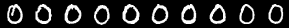
\includegraphics[width=0.9\linewidth]{predoc/images/0_ppv.png}\\
  
\includegraphics[width=0.90\linewidth]{predoc/images/1_ppv.png}\\
  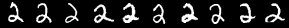
\includegraphics[width=0.90\linewidth]{predoc/images/2_ppv.png}\\
  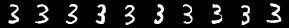
\includegraphics[width=0.90\linewidth]{predoc/images/3_ppv.png}\\
  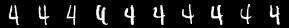
\includegraphics[width=0.90\linewidth]{predoc/images/4_ppv.png}\\
  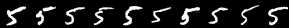
\includegraphics[width=0.90\linewidth]{predoc/images/5_ppv.png}\\
  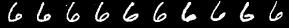
\includegraphics[width=0.90\linewidth]{predoc/images/6_ppv.png}\\
  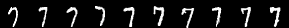
\includegraphics[width=0.90\linewidth]{predoc/images/7_ppv.png}\\
  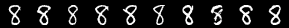
\includegraphics[width=0.90\linewidth]{predoc/images/8_ppv.png}\\
  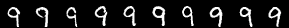
\includegraphics[width=0.90\linewidth]{predoc/images/9_ppv.png}
\end{tabular}
\end{subfigure}
\begin{subfigure}{0.45\textwidth}
% \subfigure[$10$-pca components]{
\begin{tabular}{c}
  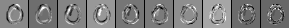
\includegraphics[width=0.9\linewidth]{predoc/images/0_eigenvectors.png}\\
  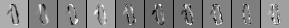
\includegraphics[width=0.90\linewidth]{predoc/images/1_eigenvectors.png}\\
  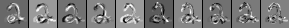
\includegraphics[width=0.90\linewidth]{predoc/images/2_eigenvectors.png}\\
  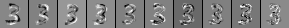
\includegraphics[width=0.90\linewidth]{predoc/images/3_eigenvectors.png}\\
  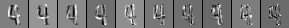
\includegraphics[width=0.90\linewidth]{predoc/images/4_eigenvectors.png}\\
  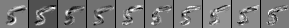
\includegraphics[width=0.90\linewidth]{predoc/images/5_eigenvectors.png}\\
  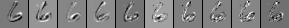
\includegraphics[width=0.90\linewidth]{predoc/images/6_eigenvectors.png}\\
  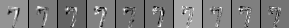
\includegraphics[width=0.90\linewidth]{predoc/images/7_eigenvectors.png}\\
  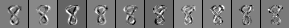
\includegraphics[width=0.90\linewidth]{predoc/images/8_eigenvectors.png}\\
  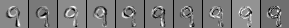
\includegraphics[width=0.90\linewidth]{predoc/images/9_eigenvectors.png}
\end{tabular}
\end{subfigure}

   \caption[Vecteurs propres d'une PCA sur les 10-ppv de classes de MNIST]{{\bf PCA Locale:} Sur MNIST, pour un exemple de chaque classe (chiffres de $0$ à $9$) on
   extrait les $10$ plus proches voisins (ppv) intra-classe et on entraîne une PCA sur cet
   ensemble. Les $10$ ppv sont présentés à gauche et les
   composantes des $10$ différentes PCA à droite. Les premières composantes de
   la PCA contiennent des informations utiles (de possibles transformations)
   tandis que les dernières n'encodent que du bruit.}

\label{fig:mnistpca}
\end{figure}

\subsection{Architectures de type Auto-Encodeur}

Nous allons maintenant présenter des méthodes non supervisées non-linéaires qui peuvent être utilisées par la suite pour
l'initialisation de réseaux de neurones.
Depuis la formalisation la plus classique de l'auto-encodeur
\textbf{(AE)}~\citep{Gallinari87} , nous présenterons le \textit{Denoising
Auto-Encoder} \textbf{(DAE)}~\citep{VincentPLarochelleH2008,Vincent-JMLR-2010}.
Ensuite, nous présenterons le \textit{Contractive Auto-Encoder}
\textbf{(CAE)}~\citep{Rifai+al-2011} et sa version d'ordre supérieur,
le \textit{Higher-Order Contractive Auto-Encoder}
\textbf{(CAE+H)}~\citep{Salah+al-2011}.

L'auto-encodeur classique se décompose en un encodeur et un décodeur.
L'encodeur le plus commun effectue une transformation affine des données paramétrisée par une
matrice de poids $W\in\mathcal{M}_{m\times d}(\mathbb{R})$ et un vecteur de biais $b\in\mathbb{R}^m$ où $m$ désigne le
nombre d'unités cachées du modèle.
Cette transformation est suivie d'une non-linéarité $s:\mathbb{R}^m \rightarrow
\mathbb{R}^m$. En général, on utilise la
fonction sigmoïde logistique $s(x)=1/(1+e^{-x})$ mais la tangente hyperbolique est aussi
communément utilisée. On a donc la forme globale suivante:

\begin{equation}
h(x)=s(Wx+b)
\end{equation}

Le décodeur tente de reconstruire l'exemple $x$ à partir de la représentation
cachée $h(x)$ et peut partager en la m\^eme matrice de poids que l'encodeur
mais a un vecteur de biais $b^{'}\in\mathbb{R}^d$ qui lui est propre. Il a
alors la forme suivante:

\begin{equation}
r(h(x))=s(W^{T} h(x)+b^{'}) \label{eq:autoenc}
\end{equation} 

La non-linéarité $s(.)$ est ici optionnelle et dépend de la nature des données
ou de la sortie désirée du décodeur par exemple si elle doit \^etre dans
l'intervalle $[0,1]$ ou non.  \\

\paragraph{Algorithme}
Tous ces paramètres sont ajustés par optimisation \textit{e.g.} descente de
gradient stochastique, visant à réduire l'erreur de reconstruction suivante:

\begin{equation}
\mathcal{J}_{\textrm{AE}} = \frac{1}{\vert \mathcal{D}\vert}\sum_{x\in\mathcal{D}_{train}}\mathcal{L}(x,r(h(x)))
\label{eq:ae}
\end{equation}

La fonction de perte $\mathcal{L}$ utilisée est en général, dans le cas de
données binaires (ou modélisant des probabilités), l'entropie croisée négative
$\mathcal{L}(x,y) = -\sum_{i=1}^d x_i\log y_i + (1-x_i)\log(1-y_i)$ ou l'erreur
quadratique $\mathcal{L}(x,y) = \| x-y\|^2_2$. Pour les fins d'initialisation
de réseaux de neurones de classification, les performances de l'auto-encodeur
classique sont largement dépassées par des versions régularisées de
l'auto-encodeur classique telles que les variantes d'auto-encodeur débruitant
(DAE) ou contractant (CAE ou CAE+H) que nous expliquerons dans les sections
suivantes.

\paragraph{Hyperparamètres} Les hyperparamètres de ce genre d'architecture sont
malheureusement nombreux. En voici une liste non exhaustive et des exemples de
valeurs typiques à raffiner par une recherche des hyperparamètres optimaux: le
nombre d'unités cachées ($1,000$), la fonction d'activation de l'encodeur ou et
du décodeur (fonction sigmoide), la fonction de perte utilisée (MSE ou Entropie
croisée), le pas de gradient ($\lbrace 10^{-1},\dots,10^{-6}\rbrace$).  \\

Une fois une certaine expertise pratique acquise avec l'entraînement de ce
genre d'architectures, l'espace des hyperparamètres à explorer qui peut
paraître exponentiellement grand au premier abord peut se réduire à quelques
valeurs.  Une astuce consiste à effectuer un échantillonage plus intelligent
d'hyper-paramètres \citep{rnn14} plutôt qu'une recherche par grille classique.

\subsubsection{Auto-Encodeur Débruitant}

On présente ici l'Auto-Encodeur Débruitant, en anglais \textit{Denoising
Auto-Encoder} (DAE)~\citep{VincentPLarochelleH2008}.  L'idée du DAE est qu'à partir de l'observation bruitée ou partielle
d'une entrée on doit être capable de reconnaître (reconstruire) l'entrée
originale. À un très haut niveau, on peut penser qu'en tant qu'êtres humains,
nous sommes capables de reconnaître des objets partiellement occultés ou aussi
bien à partir d'un son et d'une image, nous sommes en mesure de reconnaître un
film déjà vu en ne voyant que certaines séquences.  \\

Plutôt que de minimiser la perte classique Eq.~\ref{eq:ae}, on bruite artificiellement l'entrée originale
$x$ et on force l'auto-encodeur à reconstruire l'entrée originale à partir de
la version bruitée $\tilde{x}$:

\begin{equation}
\mathcal{J}_{\textrm{DAE}} = \frac{1}{\vert \mathcal{D}\vert}\sum_{x\in\mathcal{D}}\mathcal{L}(x,r(h(\tilde{x})))
\label{eq:dae}
\end{equation}

Les processus de corruption communément utilisés sont le bruit de masquage (en anglais \textit{masking noise} ou 
\textit{dropout noise})
paramétré par $p$ la probabilité de mettre à zéro une composante de l'entrée ou
le bruit gaussien paramétré par $\sigma$ où $\tilde{x} = x + \epsilon$ où
$\epsilon \sim \mathcal{N}(0,\sigma)$. D'autres types de bruit
peuvent être utilisés (voir \cite{Vincent-JMLR-2010} pour une revue).

\paragraph{Hyperparamètres} On peut citer ici en plus des hyperparamètres de
l'auto-encodeur classique le type de bruit (gaussien ou \textit{masking}) et le niveau
de bruit.

%\section{Analyse de l'effet du bruit au cours de l'apprentissage}

%Différence entre DAE et CAE. Le DAE va avoir un décodeur qui est invariant à de
%petites variations de l'entrée. Sachant que seul l'encodeur est conservé pour
%l'entraînement de réseaux de neurones, il serait préférable d'avoir le encodeur
%qui soit invariant (CAE) et non pas le décodeur (DAE). 

\subsubsection{Auto-Encodeur Contractant}

On présente ici l'Auto-Encodeur Contractant, en anglais \textit{Contractive
Auto-Encoder}~\citep{Rifai+al-2011}. Contrairement à la PCA qui extrait les
directions de variations \textbf{globales} présente dans les exemples
d'apprentissage, le CAE apprend des directions de variations \textbf{locales}.
Il suffit d'ajouter de manière explicite dans la perte minimisée
Eq.~\ref{eq:ae} une régularisation qui correspond à la norme du jacobien de
l'encodeur $h(x)$ par rapport à l'entrée $x$ sur les points de l'ensemble
d'entraînement $\mathcal{D}$:

\begin{equation}
\mathcal{J}_\textrm{CAE} = \mathcal{J}_\textrm{AE} + \lambda\frac{1}{\vert \mathcal{D}\vert}\sum_{x\in\mathcal{D}}\| \frac{\partial h}{\partial x}(x)\|_2^2
\label{eq:cae}
\end{equation}

Cette approche suggère aussi la possibilité de visualiser dans l'espace
d'entrée quelles sont les directions de variation autour d'un exemple
d'apprentissage auxquelles la représentation $h$ est sensible  (en regardant
les vecteurs propres du jacobien au point d'apprentissage). Cela permet
d'évaluer d'un point de vue qualitatif si l'extraction de caractéristiques a
convergé vers une solution intéressante ou non (voir Figure~\ref{fig:tan}).

\paragraph{Hyperparamètres} Contrairement au DAE, le CAE n'a ici qu'un seul
hyperparamètre en plus comparé à l'auto-encodeur classique. C'est le
coefficient de régularisation $\lambda$ qui va contrôler le compromis entre
erreur de reconstruction et invariance de la représentation.

\begin{figure}
\centering
\begin{subfigure}{0.9\linewidth}
%\subfigure[composantes d'une PCA sur CIFAR]
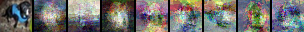
\includegraphics[width=0.9\linewidth]{predoc/images/pca.png}
\label{fig:tan_pca}
\end{subfigure}

\begin{subfigure}{0.9\linewidth}
%\subfigure[tangentes du CAE+H sur CIFAR]
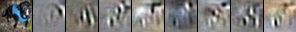
\includegraphics[width=0.9\linewidth]{predoc/images/tangents_cifar.png}
\label{fig:tan_cifar}
\end{subfigure}

\begin{subfigure}{0.9\linewidth}
%\subfigure[tangentes du CAE+H sur MNIST]
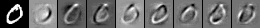
\includegraphics[width=0.9\linewidth]{predoc/images/tangents_mnist.png}
\label{fig:tan_mnist}
\end{subfigure}


   \caption[Vecteur Propres du CAE+H sur MNIST et CIFAR]{ Sur MNIST et sur CIFAR (ensemble de chiffres manuscrits/images RGB), on présente les
   tangentes apprises par le CAE+H autour d'un point d'apprentissage au milieu pour CIFAR et bas pour MNIST. On peut voir que ces
   tangentes encodent de l'information sur des transformations plausibles de
   l'image originale tandis que les composantes principales de la PCA sur CIFAR présentées en haut, n'ont
   encodé que du bruit. Pour observer les composantes de la PCA sur MNIST, nous référons à la Figure~\ref{fig:mnistpca}
\label{fig:tan}}

\end{figure}

\subsubsection{Auto-Encodeur Contractant d'Ordre Supérieur}

Si le fait de pénaliser le premier ordre de la dérivée (jacobien) de l'encodeur
par rapport à l'entrée est bénéfique, il paraît naturel d'ajouter une pénalisation
concernant les ordres supérieurs (Hessien, troisième ordre, ...) au CAE
original (Eq.~\ref{eq:cae}).  C'est l'idée présente derrière l'auto-encodeur
contractant d'ordre supérieur, en anglais \textit{Higher-order Contractive
Auto-Encoder} (CAE+H) \citep{Salah+al-2011}.  Une fois cette pénalité ajoutée
lors de l'entraînement, on pourra constater les effets obtenus en termes de
mesures quantitatives de performances de classification (bénéfique ou non) ou
de directions de variations obtenues (qualitatif).

Les pertes des Eq.~\ref{eq:ae},~\ref{eq:dae} ou~\ref{eq:cae} sont minimisées par
descente de gradient. Il est donc nécessaire de pouvoir calculer les dérivées
partielles de la perte $\mathcal{J}$ par rapport aux paramètres $\theta$. Pour commencer, le calcul de
la $k^{\textrm{ième}}$ dérivée de l'encodeur (avec $m$ unités cachées) par
rapport à l'entrée (de dimension $d$) a une complexité algorithmique de
$O(md^k)$.  Calculer les dérivées partielles de cette dérivée par rapport aux
paramètres du modèles a un coût prohibitif. Pour éviter ce calcul, on utilise donc
une approximation stochastique de la Hessienne (voir \cite{Salah+al-2011} pour
la preuve):

\begin{equation}
\|\dfrac{\partial^2 h}{\partial x^2}(x) \|_2^2 = \lim_{\sigma\rightarrow 0}\frac{1}{\sigma^2}\int_{\epsilon \rightsquigarrow \mathcal{N}(0,\sigma^2)} \| \dfrac{\partial h}{\partial x}(x) - \dfrac{\partial h}{\partial x}(x+\epsilon) \|^2_2 d\epsilon
\label{eq:hessian-approx}
\end{equation}

Si la variance $\sigma^{2}$ est non nulle, des contributions aux normes des ordres
supérieurs apparaissent \citep{Salah+al-2011}. Ces contributions disparaissent à
la limite $\sigma\rightarrow 0$. En pratique pour approximer la norme de la
Hessienne (Eq.~\ref{eq:hessian-approx}), on utilise un lot de plusieurs
versions bruitées $x+\epsilon$ du m\^eme exemple $x$ avec un $\sigma$ petit
mais non négligeable, ce qui donne lieu à l'approximation stochastique de la
norme de la Hessienne mais qui comporte aussi d'autres contributions provenant des
normes des ordres supérieurs (voir \cite{Salah+al-2011} pour plus de détails).

L'avantage d'utiliser cette approximation est que l'on peut pénaliser tous les
ordres supérieurs à un coût moindre comparé à celui d'une complexité en $O(md^k)$.
L'inconvénient est de ne plus savoir exactement quels ordres sont pénalisés et
quelle est la contribution de chacun des ordres qui permet d'apprendre de
meilleures caractéristiques. 

En utilisant cette approximation,  on aboutit à la perte du \textbf{CAE+H} avec
une taille de lot $n_c$ et $\epsilon_i \rightsquigarrow \mathcal{N}(0,\sigma)$:

\begin{equation}
\mathcal{J}_\textrm{CAE+H} = \mathcal{J}_\textrm{CAE} + \gamma\frac{1}{\vert \mathcal{D}\vert}\sum_{x\in\mathcal{D}} \frac{1}{n_c}\sum^{n_c}_{i=1} \| \dfrac{\partial h}{\partial x}(x) - \dfrac{\partial h}{\partial x}(x+\epsilon_i) \|^2_2 
\label{eq:cae}
\end{equation}

\paragraph{Hyperparamètres} Une des difficultés pratiques avec le CAE+H est son nombre
d'hyperparamètres. En plus des hyperparamètres du CAE, on a ici le coefficient
de régularisation pour les ordres supérieurs $\gamma$, le niveau de bruit
gaussien $\sigma$ et la taille du mini-lot $n_c$ utilisés pour l'estimation de
la norme de la Hessienne.

\subsubsection{Autres Méthodes d'Extraction de Caractéristiques}

Il existe de nombreuses autres méthodes d'extraction de caractéristiques qui
n'ont pas été détaillées ici. Comme méthodes d'extraction de caractéristiques
linéaires, on trouve par exemple l'analyse en composantes indépendantes, en
anglais \textit{Independent Component Analysis}~\citep{Comon94,Hyvarinen-2001}.
Cette méthode peut être utilisée pour la séparation aveugle de sources.  \\

Deux types de méthodes d'extraction de caractéristiques non-linéaire  ont aussi
fait l'objet de récentes avancées: les méthodes {\bf sparses}
\citep{ranzato-08,koray-psd-08,Koray-08} qui utilisent une pénalité sur les
activations de l'encodeur (afin de le pousser à prendre la valeur $0$ - inactif
- dans le cas d'une sigmoide)  ou les modèles {\bf génératifs} basés sur des
  fonctions d'énergie \citep{ranzato-unsup-07} comme les Machines de Boltzmann
  Restreintes, en anglais \textit{Restricted Boltzmann Machine}
  \citep{Tieleman08}.  Ces méthodes ont été utilisées avec succès pour
  l'initialisation de réseaux de neurones de type Perceptron Multi-Couches
  \citep{HintonG2006,ranzato-08,koray-psd-08,Koray-08} ou Réseaux
  convolutionnels \citep{koray-nips-10-small}. 

\subsection{Déplacement sur la Variété}
\label{sec:surfing}

D'après "l'hypothèse de variété", les distributions de données naturelles en
haute dimension seraient concentrées le long de variétés de plus faible
dimension.  En observant les vecteurs propres $V_{.i}(x)$ d'une PCA apprise à
partir de l'ensemble $\mathcal{D}_{10-ppv}(x)$ des 10 plus proches voisins d'un
point $x$ (Figure~\ref{fig:mnistpca}), on constate une similitude avec des
potentielles directions de variations autour de ce point central $x$.  Ces
directions forment un repère local orthonormé centré en ce point
$\mathcal{B}_{x}=\lbrace V_{.i}(x)~|~U_{i,i} > \epsilon\rbrace$ (voir Notation
\ref{sec:pca}). À partir de ces directions, on peut former un hyperplan tangent
local $\mathcal{H}_{x}=\lbrace x + v~|~v\in\textrm{span}(\mmathcal{B}_{x}) \rbrace$ à ce point
$x$~\citep{Dauphin-et-al-NIPS2011}.

L'hyperplan tangent local $\mathcal{H}_{x}$ est un nouvel ensemble de points
localement proches de la variété le long de laquelle se concentrent les
exemples d'apprentissage au voisinage du point $x$.  À partir de cette idée, on
peut imaginer naviguer sur la variété de proche en proche (d'un point
suffisamment proche d'un autre) en suivant ces directions de variations et en
"reprojetant" au besoin sur la variété à l'aide d'un auto-encodeur qui la
modélise.

Si on suppose que la variété peut être approximée localement de façon linéaire
entre deux points suffisamment proches, cela évite d'essayer de "connecter"
deux points $x_i$ et $x_j$ par des directions provenant des hyperplans tangents
$\mathcal{H}_{x_i}$ et $\mathcal{H}_{x_j}$. On effectue plutôt le mouvement par une
simple interpolation linéaire entre les deux points voisins $x_{i}$ et $x_{j}$~\citep{Mesnil-et-al-LW2012}.

\begin{equation}
x_{i,j,\alpha} = x_{i} + \alpha (x_{i} - x_{j})
\end{equation}

avec $\alpha \in ]0,1[$. Il est aussi possible d'effectuer une approximation
non-linéaire de la variété si cette interpolation a lieu dans l'espace des
représentations $h(x)$ et que l'on revient dans l'espace original des $x$ par une
simple reconstruction du décodeur. Avec la notation de l'équation
\ref{eq:autoenc}, on obtient:

\begin{equation}
x_{i,j,\alpha} = r(h(x_{i}) + \alpha h(x_{i}) - h(x_{j})))
\end{equation}

Dans le Chapitre~\ref{chap:mixing}, on montrera qu'il est plus aisé de se déplacer sur la
variété à partir des représentations $h(x)$. Nous montrerons également 
qu'il est plus facile de mixer (de passer d'une classe à l'autre)
lors du processus d'échantillonnage pour les CAEs ou RBMs si l'échantillonnage a lieu dans
l'espace des représentations apprises $h(x)$ plutôt que dans l'espace
original des données $x$.

\subsection{Transfert de Domaine: PCA Transductive et Finetuning}

Dans les sections précédentes, nous avons toujours supposé que les données dans
$\mathcal{D}_{train}$, $\mathcal{D}_{valid}$ et $\mathcal{D}_{test}$
provenaient de la même distribution. Dans le paradigme du transfert de domaine,
cette hypothèse n'est plus valable. Cependant, ce n'est pas pour autant qu'il
faut reconstruire les ensembles de données afin de satisfaire cette
contrainte de distribution identique. Il est plus intelligent de proposer un
apprentissage transductif afin de pouvoir transférer nos connaissances apprises
à partir de $\mathcal{D}_{train}$ sur les ensembles $\mathcal{D}_{valid}$ et
$\mathcal{D}_{test}$. Le transfert d'apprentissage transductif suppose que la
distribution sous-jacente à $\mathcal{D}_{valid}$ et $\mathcal{D}_{test}$
partage de manière limitée ou non le support de la distribution sous-jacente à
$\mathcal{D}_{train}$. Pour une revue complète des différents types de
transfert d'apprentissage (inductif, non supervisé et transductif), on réfère
le lecteur à la revue de littérature sur ce sujet par \citep{Pan-transfer}.

\subsubsection{PCA Transductive}

Cette approche est transductive et suppose donc que les variations des exemples
dans $\mathcal{D}_{valid}$ ou $\mathcal{D}_{test}$ sont un sous-ensemble des
variations de $\mathcal{D}_{train}$.  Nous pouvons imaginer un exemple comme
nous verrons dans le Chapitre \ref{chap:utlc} où $\mathcal{D}_{train}$
contiendrait toutes les images de chiffres $\lbrace 0,\dots,9 \rbrace$ tandis
que l'ensemble $\mathcal{D}_{valid}$ contiendrait seulement les chiffres
$\lbrace 0,1,2 \rbrace$ et $\mathcal{D}_{test}$ les chiffres $\lbrace 5,6,7
\rbrace$.

La PCA transductive n'est pas entraînée à partir de $\mathcal{D}_{train}$. Une
fois que le processus d'apprentissage non-supervisé de $h(x)$ sur l'ensemble
$\mathcal{D}_{train}$ est achevé, on entraîne la PCA transductive sur la
représentation apprise $h(x)$ avec $x\in\mathcal{D}_{valid}$ ou
$x\in\mathcal{D}_{test}$. On entraîne une PCA par ensemble, il y aura donc deux
PCA à apprendre dans ce cas. En comparant la notation dans la Section $\ref{sec:pca}$, cela
revient à remplacer $X$ par $\lbrace h(x)~|~x\in\mathcal{D}_{valid}\rbrace$ ou
$\lbrace h(x)~|~x\in\mathcal{D}_{test}\rbrace$ suivant l'ensemble pour lequel
on veut obtenir la représentation.

La PCA transductive a pour objectif de ne retenir que les variations dominantes
dans la représentation des ensembles $\mathcal{D}_{valid}$ ou
$\mathcal{D}_{test}$. Le classifieur utilisé à partir de la représentation
$h(x)$ pourra ainsi ignorer les variations présentes dans $\mathcal{D}_{train}$
sans intérêt pour $\mathcal{D}_{valid}$ ou $\mathcal{D}_{test}$ pour ne se
concentrer que sur celles présentes dans les ensembles $\mathcal{D}_{valid}$ ou
$\mathcal{D}_{test}$. On peut assimiler ces variations "en trop" à du bruit. La
représentation $h(x)$ conserve donc toutes les variations jusqu'à la PCA
transductive apprise à partir de $h(x)$ qui elle, ne se concentre que sur les
variations spécifiques à l'ensemble de données en question,
$\mathcal{D}_{valid}$ ou $\mathcal{D}_{test}$. 

\subsubsection{Finetuning}

Nous disposons d'une masse de données non labelées considérable sur le web.
Lorsque notre ensemble de données labelées $\mathcal{D}_{small-labeled}$ est de
quatité réduite, il peut être intéressant d'apprendre une représentation non
supervisé sur un grand ensemble de données non labelées
$\mathcal{D}_{big-unlabeled}$ partageant les mêmes structures que les données
de $\mathcal{D}_{small-labeled}$, par exemples ces données sont toutes des
images d'objets. Par la suite cette représentation est utilisée comme point
d'initialisation pour un apprentissage supervisé d'un réseau de neurones
profond. On peut alors parler de transfert de connaissances apprises sur un
grand ensemble de données $\mathcal{D}_{big-unlabeled}$ à un plus petit
ensemble $\mathcal{D}_{small-labeled}$.  Nous verrons que cela permet d'obtenir
des gains significatifs de performance pour la classification d'images de
scènes (Chapitre \ref{chap:ob}).

\section{Classification de Séquences}

Les réseaux de neurones peuvent aussi être utilisés pour la classification de
séquences, on utilise en général dans ce cas des réseaux de neurones récurrents.
Dans le cadre de l'apprentissage supervisé simple
(Section~\ref{sec:supervised}), nos ensembles $\mathcal{D}_{train}$,
$\mathcal{D}_{valid}$ et  $\mathcal{D}_{test}$  sont composés des entrées
$x\in\mathbb{R}^{d}$ et un label $y\in\{1,\dots ,C\}$ qui leur est associé.
Pour la classification de séquences, les données sont séquentielles et pour une
séquence de longueur $T$, on a $x=\lbrace x_{i}\in\mathbb{R}^{d}
\rbrace_{i=1}^{T}$ et $y=\lbrace y_{i}\in\{1,\dots ,C\}_{i=1}^{T}\}$.

En traitement du langage naturel par exemple (Chapitre \ref{chap:rnn}), chaque
entrée est une séquence de mots et le label $y$ est constitué d'une séquence de
classes associées à chacun des mots (Figure \ref{fig:iob}). À noter que la
longueur $T$ de la séquence n'est pas uniforme dans l'ensemble de données et
peut varier.

\subsection{Conditional Random Fields}

Une des méthodes de classification de séquences les plus utilisées sont les CRFs \citep{rnn6} et leurs variantes.
La probabilité conditionnelle de modéliser une sortie $y$ conditionnellement à
$x$ pour une chaîne linéaire s'écrit sous la forme suivante:

\begin{equation}
f_{\theta}(y~\vert~x) = \frac{1}{Z(x)}\prod_{t=1}^{T}\exp{H(y_{t-1}, y_{t}, x_{t}})
\end{equation}

avec $Z(x)$ un facteur de normalisation et les $M$ fonctions $h_{m}(y_{t-1},
y_{t}, x_{t})$ "caractéristique" sont définies de la manière suivante:

\begin{equation}
H(y_{t-1}, y_{t}, x_{t}) = \sum_{m=1}^{M}\lambda_{m}h_{m}(y_{t-1}, y_{t}, x_{t})
\end{equation}

Les fonctions $h_{m}$ sont fixées au départ et l'apprentissage consiste à
ajuster les $\lambda_{m}$. Une fonction caractéristique peut prendre la forme
suivante par exemple:

\begin{equation}
h_{m}(y_{t-1}, y_{t}, x_{t}) = 
\left\{
\begin{split}
1 &  \textrm{~si $x_{t}$ = "september", $y_{t-1}$ = "chiffre" et $y_{t}$ = "mois"} \\ 
0 & \textrm{~sinon}
\end{split}
\right.
\end{equation}

L'apprentissage s'effectue par l'ajustement des paramètres $\theta=\lbrace
\lambda_m \rbrace_{m=1}^{M}$ pour maximiser la log-vraisemblance sur l'ensemble
$\mathcal{D}_{train}$:

\begin{equation}
\mathcal{J}_{\textrm{CRF}} =\sum_{(x,y)\in\mathcal{D}_{train}} \sum_{t=1}^{T} \log (\dfrac{1}{Z(x_{t})}) + \sum_{m=1}^{M} \lambda_{m} h_{m}(y_{t-1}, y_{t}, x_{t})
\label{eq:loglikecrf}
\end{equation}

L'équation \ref{eq:loglikecrf} est différentiable par rapport à $\theta=\lbrace
\lambda_m \rbrace_{m=1}^{M}$ et concave. Il n'y a donc qu'un seul maximum et on
peut l'approcher par des méthodes à base de gradient.

\subsection{Réseaux de Neurones Récurrents}

Les réseaux de neurones récurrents sont des architectures profondes. Si on
compare aux architectures profondes habituelles à $m$ couches, la rétro-propagation
du gradient au travers des $m$ couches revient à effectuer une
rétro-propagation dans le temps pour $m$ unités de temps dans le passé.

L'architecture de réseau récurrent de base \citep{rnn16} garde une trace des
représentations du passé au travers de ses connections récurrentes.  La
représentation $h_{t}(x)$ peut donc être vue comme un résumé des états
précédents $\lbrace h_{k}(x)\rbrace_{k=0}^{t-1}$.

Il existe plusieurs architectures de réseaux de neurones récurrents possibles
(Elman, Jordan, uni-directionnel, bi-directionnel) \citep{rnn15}, nous
décrivons ici la forme la plus simple. Pour un RNN de type Elman pour une séquence
d'entrées $\lbrace x_{i}\in\mathbb{R}^{d}\rbrace_{i=1}^{T}$ on a la
représentation $\lbrace h_{i}(x)\in\mathbb{R}^{d_h}\rbrace_{i=1}^{T}$ à $d_h$
unités cachées suivante:

\begin{equation}
h_t(x) = s(Ux_{t}+Vh_{t-1}(x))
\end{equation}

paramétré par $U\in\mathcal{M}_{d_h\times d}(\mathbb{R})$,
$V\in\mathcal{M}_{d_h\times d_h}(\mathbb{R})$ et $h_{0}\in\mathbb{R}^{d_h}$.

Pour effectuer la prédiction, on ajoute la couche supérieure suivante similaire à l'équation \ref{eq:softmax}:

\begin{equation}
f_{t}(x) = \frac{e^{ h_{t}(x) + b}}{\sum_{j=1}^C e^{W_{j.} h_{t}(x) + b_{j} }} \in [0,1]^{C}
\end{equation}

Pour entraîner le modèle, on effectue une minimisation par descente de gradient
de la log-vraisemblance négative pour chaque séquence de $\mathcal{D}_{train}$:

\begin{equation}
\label{eq:nll-rnn}
\mathcal{J}(\theta) = - \sum_{(x,y)\in\mathcal{D}_{train}} \sum_{t=1}^{T}\log f_{t}(x_{t})_{y_{t}}
\end{equation}

pour les paramètres $\theta=\lbrace U, V, W, b, h_{0}\rbrace$. Pour obtenir
l'équation \ref{eq:nll-rnn} précédente, l'hypothèse d'indépendance
conditionnelle des $y_i$ sachant $x$ a été faite.
